\documentclass[11pt,a4paper]{article}

% ============================================================
% Packages
% ============================================================
\usepackage[margin=1in]{geometry}
\usepackage{amsmath,amssymb}
\usepackage{graphicx}
\usepackage{booktabs}
\usepackage{hyperref}
\usepackage{natbib}
\usepackage{algorithm}
\usepackage{algorithmic}
\usepackage{xcolor}
\usepackage{multirow}
\usepackage{listings}
\usepackage{caption}
\usepackage{subcaption}
\usepackage{float}

% ============================================================
% Code listing settings for Appendix A
% ============================================================
\lstset{
    basicstyle=\ttfamily\small,
    breaklines=true,
    frame=single,
    numbers=left,
    numberstyle=\tiny,
    keywordstyle=\color{blue},
    commentstyle=\color{green!60!black},
    stringstyle=\color{red},
    showstringspaces=false
}

% ============================================================
% Document
% ============================================================
\begin{document}

% ============================================================
% Title and Abstract
% ============================================================
\title{LW-AdaDelta: A Local-Window Adaptive Optimizer for Non-Stationary Gradient Landscapes}
\author{Razi-ur-Rehman Khan\\
\small{Independent Researcher}}
\date{\today}

\maketitle

\begin{abstract}
Adaptive optimizers maintain running estimates of gradient statistics over the full training history. In non-stationary settings---such as noisy labels, distribution shift, or long temporal dependencies---this infinite accumulation causes gradient scale estimates to become stale, reducing the optimizer's ability to respond to recent signal.

We propose \textbf{Locally Weighted AdaDelta (LW-AdaDelta)}, a modification that replaces global accumulation with a fixed-size window of recent gradients. Within this window, gradients are weighted using exponential decay, giving greater importance to recent updates while preserving short-term history; gradients outside the window are discarded entirely. This design enables faster adaptation to changing gradient dynamics while retaining the normalization benefits of adaptive methods.

We evaluate LW-AdaDelta on six benchmark datasets spanning noisy classification, outlier-robust regression, and temporal forecasting. We compare against SGD, Adam, AdamW, Lion, and AdaDelta using their standard published hyperparameters. LW-AdaDelta consistently outperforms these baselines, achieving a +1.58\% accuracy gain on CIFAR-10 with 40\% label noise, a 16.2\% reduction in MAE on ETTh1 (H=48), and a 5.4\% MAE improvement with 20$\times$ lower variance on the NYC Taxi dataset. Additionally, it demonstrates consistently lower seed-to-seed variance across all benchmarks.

These results indicate that LW-AdaDelta provides a practical and robust optimization strategy for non-stationary learning environments. Notably, it achieves these gains without dataset-specific hyperparameter tuning; the same default settings ($\rho = 0.9$, $k = 2$, $\tau = 1.0$) are used across all experiments, making it particularly suitable for real-world applications where tuning is costly.
\end{abstract}

% ============================================================
% 1. Introduction
% ============================================================
\section{Introduction}

Optimization lies at the heart of deep learning, directly influencing convergence speed, final accuracy, and robustness to difficult training conditions. As models and datasets grow in complexity, the choice of optimization algorithm has become increasingly consequential, motivating sustained research into methods that are both effective and practical.

Adaptive gradient methods emerged as a response to the limitations of stochastic gradient descent, which applies a uniform learning rate across all parameters regardless of their individual gradient histories. Methods such as AdaGrad \citep{duchi2011adagrad}, RMSProp \citep{tieleman2012rmsprop}, Adam \citep{kingma2014adam}, and AdaDelta \citep{zeiler2012adadelta} addressed this by accumulating gradient statistics to automatically scale updates on a per-parameter basis. Among these, AdaDelta stands out for eliminating the need for a manually specified global learning rate entirely, relying instead on two running averages of squared gradients and squared parameter updates. This property made AdaDelta particularly attractive in practice, as it reduces the burden of hyperparameter tuning that accompanies most other adaptive methods.

Despite their widespread adoption, adaptive optimizers share a fundamental assumption that gradient distributions remain approximately stationary throughout training. In practice this assumption is routinely violated. Non-stationarity arises from multiple sources: label noise corrupts gradient signals in classification tasks, outliers introduce high-magnitude updates in regression settings, temporal dependencies cause gradient character to shift across batches, and data augmentation ensures that no two gradient estimates are identical. When gradient distributions shift substantially, the accumulated historical statistics that drive adaptive methods become misleading. Step sizes computed from stale history may be poorly calibrated to the current loss landscape, causing the optimizer to take suboptimal steps precisely when reliable adaptation is most critical.

AdaDelta is particularly susceptible to this failure mode. Its infinite exponential moving average means that gradient statistics from early training---potentially computed under very different data conditions---continue to influence parameter updates throughout the entire training process. When early gradients are corrupted or unrepresentative, this persistent influence degrades the quality of later updates in ways that cannot be corrected without restarting training.

Existing approaches to this problem typically operate at the learning rate schedule level, employing warm-up strategies, cyclical schedules, or adaptive restarts \citep{loshchilov2016cosine}. While these methods can partially compensate for non-stationarity, they do not address the underlying cause: the accumulation mechanism itself. To our knowledge no prior work has directly targeted stale gradient history by modifying the accumulation window within the AdaDelta framework.

This observation motivates our proposed method, Locally Weighted AdaDelta (LW-AdaDelta). Rather than accumulating gradients over the full training history, LW-AdaDelta maintains a fixed-size window of the $k$ most recent gradient updates. Within this window, contributions are weighted using exponential decay, ensuring that more recent gradient information exerts greater influence on parameter updates while older information within the window provides diminishing but non-zero context. Gradients outside the window are discarded entirely, preventing early corrupted statistics from persisting into later training stages. Critically, LW-AdaDelta preserves the hyperparameter-free philosophy of its predecessor---the same default values ($\rho = 0.9$, $k = 2$, $\tau = 1.0$) are used across all experiments without dataset-specific tuning.

This paper makes the following contributions:
\begin{enumerate}
    \item We propose LW-AdaDelta, a modification of AdaDelta that replaces infinite gradient accumulation with a finite local window of size $k$, weighted by exponential decay.
    \item We provide a mechanistic analysis of why local windowing improves optimizer performance under non-stationary gradient conditions.
    \item We evaluate LW-AdaDelta across six real-world benchmarks spanning diverse challenging conditions including noisy labels, outlier contamination, temporal forecasting, and skewed regression, demonstrating consistent improvements over AdaDelta and competitive performance against five widely used optimizers.
    \item We show that LW-AdaDelta exhibits consistently lower seed-to-seed variance across all benchmarks, offering improved training stability without requiring hyperparameter tuning.
\end{enumerate}

The remainder of this paper is organised as follows. Section~\ref{sec:related} reviews related work on adaptive optimization and identifies the gap that LW-AdaDelta addresses. Section~\ref{sec:methodology} presents the methodology and formal algorithm. Section~\ref{sec:experimental} describes the experimental setup. Section~\ref{sec:results} presents results and analysis. Section~\ref{sec:discussion} discusses broader implications and limitations, and Section~\ref{sec:conclusion} concludes.

% ============================================================
% 2. Related Work
% ============================================================
\section{Related Work}
\label{sec:related}

\subsection{Adaptive Optimization Methods}

The realization that a single global learning rate is inadequate for training deep neural networks with diverse parameter scales has propelled the advancement of adaptive optimization methods. AdaGrad \citep{duchi2011adagrad} introduced per-parameter learning rate adaptation by summing the squared gradients, which lowered the learning rate for parameters that were updated often and raised it for parameters that weren't. AdaGrad works well in sparse gradient settings, but its learning rates keep going down, which can make them very small before convergence is reached.

RMSProp \citep{tieleman2012rmsprop} fixed this problem by using an exponential moving average of squared gradients instead of the cumulative sum. This stopped the learning rate from going down to zero. This change added a decay hyperparameter that controls how quickly old gradient information is forgotten. However, practitioners still had to choose this parameter manually.

AdaDelta \citep{zeiler2012adadelta} built on the idea of RMSProp by getting rid of the global learning rate completely. AdaDelta didn't just scale gradients by a running average of squared gradients. Instead, it added a second running average that tracked squared parameter updates, which made a ratio that was close to a diagonal Hessian and gave updates that were consistent in all dimensions. This design made AdaDelta one of the first truly hyperparameter-reduced adaptive optimizers. It only needed a decay rate $\rho$ that worked well on a lot of different tasks without any tuning.

Adam \citep{kingma2014adam} merged the momentum of RMSProp with first and second moment estimates that had been corrected for bias, making it the most popular optimizer in deep learning. Because it worked so well, many different versions were made, such as AdamW \citep{loshchilov2017adamw}, which separates weight decay from the gradient update to make regularization better, and AMSGrad \citep{reddi2018amsgrad}, which keeps a running maximum of second moment estimates instead of a simple moving average to deal with convergence issues.

Lion \citep{chen2023lion} recently came up with a sign-based update rule using evolutionary search. It works just as well as Adam-family methods but uses much less memory. These changes are part of a bigger trend toward optimizers that find a balance between adaptation and computational efficiency.

\subsection{Non-Stationarity in Optimization}

Most theoretical studies of adaptive optimizers are based on the idea that gradient distributions are stationary. In practice, gradient distributions change a lot during training because the data distributions change, the model representations change, and regularization and augmentation strategies have an effect. A number of studies have recognized non-stationarity as a significant obstacle for adaptive methods, observing that aggregated statistics calculated during the initial phases of training may progressively diverge from the prevailing optimization landscape.

Warm-up strategies deal with instability in early training by slowly raising the learning rate. This stops big updates from messing up gradient statistics before the model has reached a stable regime. Cosine annealing and cyclical learning rates \citep{loshchilov2016cosine} are two types of learning rate schedules that periodically reset or lower the learning rate to get out of optimization paths that are no longer useful. Gradient clipping \citep{pascanu2013clipping} keeps the size of each update small so that outlier gradients don't mess up the statistics that have been built up. These methods only partially fix the problem because they only work on the size of updates and not the way they are stored. This means that the main problem of old statistics is still not fixed.

Research on continual learning has investigated non-stationarity most explicitly, as models in this context must adjust to authentically varying task distributions over time. Elastic weight consolidation \citep{kirkpatrick2017ewc} and gradient episodic memory are two methods that keep important parameters from being overwritten by new gradient data. But these methods are meant for clear task boundaries, not the continuous gradient non-stationarity that happens during a single training run.

\subsection{Local and Windowed Gradient Methods}

Gradient statistics over a sliding window were employed in the field of online learning and algorithms are shown to have regret bounds based on a sliding window-based statistical methodology for obtaining gradient descent updates. In deep learning applications, several papers have proposed alternative means for weighting the latest gradients in the adaptive learning methods. For example, Padam \citep{chen2018padam} and some of its extensions use interpolation techniques to balance the degree of adaptivity with the degree of convergence assurance for accumulated gradient descent updates, by controlling for the total amount of historical gradients available (i.e., partial vs full gradient accumulations). Other examples of this type of gradient weighting are to use slow and fast copies of parameters through a method called Lookahead \citep{zhang2019lookahead}, which allows for a form of temporal windowing on the parameter-level rather than the statistical-level based on the accumulated historical number of gradients available.

No prior work has directly applied fixed-size local windowing to AdaDelta's accumulation mechanism and evaluated the result across diverse non-stationary benchmarks. As a result, LW-AdaDelta was developed to fill this gap by replacing AdaDelta's infinite memory with a fixed-size, local temporal window for its accumulated gradients while preserving the hyperparameter-free nature of AdaDelta's framework.

% ============================================================
% 3. Methodology
% ============================================================
\section{Methodology}
\label{sec:methodology}

\subsection{AdaDelta Revisited}

AdaDelta is an adaptive learning rate method that tries to resolve SGD's two main issues:
\begin{enumerate}
    \item SGD's sensitivity to learning rate hyperparameter
    \item Different scales of gradients across parameters
\end{enumerate}

AdaDelta removes the need of manual learning rate replacing it with two running averages, eliminating need for hyperparameter tuning.

\subsubsection{The Two Running Averages}

\textbf{1. $E[g^2]_t$ --- Running average of squared gradients}

Tracks the magnitude of recent gradients (momentum-like for second moment):
\begin{equation}
E[g^2]_t = \rho E[g^2]_{t-1} + (1-\rho) g_t^2
\end{equation}
where $g_t = \nabla_\theta J(\theta_t)$ (gradient at step $t$), $\rho$ is a decay constant (typically 0.95), and $E[g^2]_0 = 0$.

\textbf{2. $E[\Delta x^2]_t$ --- Running average of squared parameter updates}

Tracks the magnitude of recent updates (acts as a local estimate of curvature):
\begin{equation}
E[\Delta x^2]_t = \rho E[\Delta x^2]_{t-1} + (1-\rho) \Delta x_t^2
\end{equation}
where $\Delta x_t = x_t - x_{t-1}$ (parameter update from previous step) and $E[\Delta x^2]_0 = 0$.

\subsubsection{Update Rule}

The parameter update at time $t$ is:
\begin{equation}
\Delta x_t = - \frac{\sqrt{E[\Delta x^2]_{t-1} + \epsilon}}{\sqrt{E[g^2]_t + \epsilon}} g_t, \qquad x_{t+1} = x_t + \Delta x_t
\end{equation}
where $\epsilon$ is a small constant (e.g., $10^{-6}$ or $10^{-8}$) for numerical stability.

\subsection{The Stale Gradient Problem}

The running average $E[g^2]_t$ can be expressed as a weighted sum:
\begin{equation}
E[g^2]_t = (1-\rho) \sum_{i=1}^t \rho^{t-i} g_i^2
\end{equation}

The weight on gradient at step $i$ when computing $E[g^2]_t$ is $w_{t,i} = (1-\rho) \cdot \rho^{t-i}$. As $t \rightarrow \infty$, older gradients retain non-zero weights indefinitely. This is the specific mechanism we are trying to fix.

\subsection{LW-AdaDelta: Local-Window Weighting}

Unlike standard AdaDelta that uses exponential moving averages for both gradient and statistics, we propose LW-AdaDelta that:
\begin{enumerate}
    \item \textbf{Maintains a finite buffer} of the $k$ most recent \textbf{raw updates} $\Delta\theta^{\text{raw}}$
    \item \textbf{Smooths across this local window} using exponentially decaying weights
    \item \textbf{Preserves AdaDelta's dimensional consistency} while adding a controllable temporal horizon
\end{enumerate}

\subsubsection{Mathematical Formulation}

\textbf{1. Gradient Accumulation (Same as AdaDelta)}
\begin{equation}
E[g^2]_t = \rho E[g^2]_{t-1} + (1-\rho) g_t^2
\end{equation}

\textbf{2. Raw Update Calculation (Same as AdaDelta)}
\begin{equation}
\Delta\theta_t^{\text{raw}} = - \frac{\sqrt{E[\Delta\theta^2]_{t-1}} + \epsilon}{\sqrt{E[g^2]_t} + \epsilon} g_t
\end{equation}

\textbf{3. Update Accumulation for Unit Consistency (Same as AdaDelta)}
\begin{equation}
E[\Delta\theta^2]_t = \rho E[\Delta\theta^2]_{t-1} + (1-\rho)(\Delta\theta_t^{\text{raw}})^2
\end{equation}

\textbf{4. Local Window Definition}
\begin{equation}
\mathcal{U}_t = \{\Delta\theta_t^{\text{raw}}, \Delta\theta_{t-1}^{\text{raw}}, \ldots, \Delta\theta_{t-k+1}^{\text{raw}}\}
\end{equation}

\textbf{5. Weight Computation (Exponential Decay within Window)}
For a window of size $k$ with decay parameter $\tau > 0$:
\begin{equation}
\alpha_i = \frac{\exp(-i/\tau)}{\sum_{j=0}^{k-1} \exp(-j/\tau)}, \quad i = 0,1,\ldots,k-1
\end{equation}
where $i = 0$ corresponds to the \textbf{most recent} raw update $\Delta\theta_t^{\text{raw}}$.

Properties:
\begin{itemize}
    \item $\sum_{i=0}^{k-1} \alpha_i = 1$
    \item $\alpha_0 > \alpha_1 > \cdots > \alpha_{k-1} > 0$
    \item As $\tau \rightarrow \infty$, $\alpha_i \rightarrow 1/k$ (uniform weights)
    \item As $\tau \rightarrow 0$, $\alpha_0 \rightarrow 1$, others $\rightarrow 0$ (no smoothing)
\end{itemize}

\textbf{6. Final Parameter Update (Weighted Combination)}
\begin{equation}
\Delta\theta_t = \sum_{i=0}^{k-1} \alpha_i \Delta\theta_{t-i}^{\text{raw}}, \qquad \theta_{t+1} = \theta_t + \Delta\theta_t
\end{equation}

\subsection{Algorithm}

\begin{algorithm}[H]
\caption{LW-AdaDelta (Local Window AdaDelta)}
\begin{algorithmic}[1]
\REQUIRE $\rho \in (0,1)$, $\epsilon > 0$, $\tau > 0$, $k \in \mathbb{N}$, $\theta_0$, $T$
\ENSURE $\theta_T$ (optimized parameters)

\STATE Initialize $E[g^2]_{-1} = 0$, $E[\Delta\theta^2]_{-1} = 0$
\STATE Buffer $\mathcal{U} = \text{empty list}$ (max size $k$)

\FOR{$t = 0, 1, 2, \ldots, T-1$}
    \STATE $g_t \leftarrow \nabla_\theta \mathcal{L}(\theta_t)$
    \STATE $E[g^2]_t \leftarrow \rho \cdot E[g^2]_{t-1} + (1-\rho) \cdot g_t^2$
    \STATE $\Delta\theta_t^{\text{raw}} \leftarrow - \frac{\sqrt{E[\Delta\theta^2]_{t-1}} + \epsilon}{\sqrt{E[g^2]_t} + \epsilon} \cdot g_t$
    \STATE $E[\Delta\theta^2]_t \leftarrow \rho \cdot E[\Delta\theta^2]_{t-1} + (1-\rho) \cdot (\Delta\theta_t^{\text{raw}})^2$
    \STATE $\mathcal{U} \leftarrow \mathcal{U} \cup \{\Delta\theta_t^{\text{raw}}\}$
    \IF{$|\mathcal{U}| > k$}
        \STATE $\mathcal{U} \leftarrow \mathcal{U} \setminus \{\text{oldest element}\}$
    \ENDIF
    \STATE $\alpha_i \leftarrow \frac{\exp(-i/\tau)}{\sum_{j=0}^{|\mathcal{U}|-1} \exp(-j/\tau)}, \quad i = 0,\ldots,|\mathcal{U}|-1$
    \STATE $\Delta\theta_t \leftarrow \sum_{i=0}^{|\mathcal{U}|-1} \alpha_i \cdot \mathcal{U}[i]$
    \STATE $\theta_{t+1} \leftarrow \theta_t + \Delta\theta_t$
\ENDFOR
\end{algorithmic}
\end{algorithm}

\subsection{Hyperparameter Discussion}

Hyperparameters of LW-AdaDelta were selected to achieve levels of simplicity and interpretability without sacrificing performance on different types of tasks. The size of the window, $k=2$, is the smallest configuration that captures local temporal structure that is not limited to 1 step (allowing for a weighted combination of the current raw update with the most recent raw update while avoiding excessive computational load and potential excessive smoothing of larger window sizes). The decay parameter, $\tau=1.0$, produces a recency bias for the most recent raw updates while still maintaining significant influence from earlier raw updates, $\alpha_0 \approx 0.731$ and $\alpha_1 \approx 0.269$, through the following weighting. The value of the recurrent decay parameter, $\rho=0.9$, was inherited from standard AdaDelta without retuning as it is well understood to regulate the effective history of squared gradients and squared updates. We recognize that while hyperparameters could have been optimized for each task, we purposely kept them fixed across all experiments to show that LW-AdaDelta is a robust design. A preliminary sensitivity analysis (Appendix C) suggests performance is stable for $k \in \{2,3,4\}$ and $\tau \in [0.5,2.0]$.

\subsection{Computational Complexity}

\textbf{Memory:} Standard AdaDelta maintains two accumulators per parameter: $E[g^2]$ and $E[\Delta\theta^2]$. LW-AdaDelta adds a buffer of $k$ raw updates per parameter, requiring $O(k)$ additional memory. At $k = 2$, this doubles the buffer storage but remains $O(1)$ with respect to the number of training steps.

\textbf{Computation:} The weighted combination $\Delta\theta_t = \sum_{i=0}^{k-1} \alpha_i \Delta\theta_{t-i}^{\text{raw}}$ adds $O(k)$ operations per parameter. For $k = 2$, this is one additional multiply-add per parameter per iteration---negligible compared to the cost of gradient computation.

\textbf{Connection to AdaDelta:} As $k \rightarrow \infty$ and weights become uniform ($\tau \rightarrow \infty$), LW-AdaDelta's weighted window average converges to standard AdaDelta's infinite EMA, establishing LW-AdaDelta as a strict generalization.

% ============================================================
% 4. Experimental Setup
% ============================================================
\section{Experimental Setup}
\label{sec:experimental}

\subsection{Initial Screening Study (30 Synthetic Datasets)}

To identify suitable benchmark datasets and validate LW-AdaDelta's design choices, we first ran a screening study across 30 synthetic datasets from six categories: short and smooth (5 datasets), short and high variance (5), long sequences (5), sparse features (5), NLP-like tasks (5), and regression (5). We evaluated each dataset using six optimizers (SGD, Adam, AdamW, Lion, AdaDelta, LW-AdaDelta) across five random seeds for 60 to 80 training epochs. The results, summarized in Appendix Table X, led us to select $k=2$ and $\tau=1.0$ as the default LW-AdaDelta settings. These consistently outperformed other window sizes ($k \in \{1,3,4\}$) and decay parameters ($\tau \in \{0.5,2.0\}$) in non-stationary task categories. From this screening, we chose six real-world benchmarks that feature the most challenging non-stationary gradient landscapes for the main evaluation.

\subsection{Main Benchmark Datasets (6 total)}

\paragraph{CIFAR-10 with Label Noise.} CIFAR-10 \citep{krizhevsky2009cifar} includes 60,000 color images sized $32 \times 32$ across 10 classes (50,000 for training, 10,000 for testing). Label noise introduces non-stationary gradient statistics as the model first learns clean patterns and then must adjust to corrupted labels. This makes it a good test for how well optimizers handle sudden changes in the landscape. The task is multi-class classification, and accuracy is the main metric. We evaluate with 20\% and 40\% symmetric label noise rates.

\paragraph{California Housing with Injected Outliers.} This dataset \citep{pace1997california} contains 20,640 blocks from the 1990 California census with eight numerical features used to predict median house value. We inject outliers at rates of 10\% and 15\% (with magnitudes of $3\sigma$, $4\sigma$, $5\sigma$) to simulate sudden gradient spikes typical of non-stationary regression problems. The task is regression, evaluated using MAE and MedAE.

\paragraph{UCI HAR (Human Activity Recognition).} UCI HAR \citep{anguita2013ucihar} consists of 10,299 smartphone sensor readings from 30 subjects carrying out six activities (walking, walking upstairs, downstairs, sitting, standing, lying down). The multi-subject setup naturally creates non-stationarity, as the model must adapt to different movement patterns. The task is multi-class classification, with macro F1 as the main metric.

\paragraph{ETT Load Forecasting (ETTh1 + ETTh2).} The Electricity Transformer Temperature dataset \citep{zhou2021informer} includes oil temperature readings from two Chinese power transformers (ETTh1, ETTh2) collected over two years. Time series forecasting, influenced by seasonal shifts and holiday effects, creates realistic non-stationary conditions. The task involves multi-step forecasting at 24h, 48h, and 168h horizons using a sequence length of 336, evaluated with MAE and RMSE.

\paragraph{NYC Taxi Fare.} This synthetic dataset retains the statistical characteristics (spatial distribution, temporal patterns, outlier frequencies) of real NYC taxi trip data from 2009 to 2015. The synthetic generation allows us to control non-stationarity while keeping it realistic. The task is to regress fare amounts using MAE, MedAE, and R$^2$ metrics.

\paragraph{PTB-XL ECG.} PTB-XL \citep{wagner2020ptbxl} includes 21,837 12-lead ECG recordings, each lasting 10 seconds (1,000 timesteps), from 18,885 patients, labeled across five diagnostic categories. Variability in heart signals from patient to patient and age-related changes add natural non-stationarity to the input distribution. The task is multi-class classification, evaluated primarily with macro AUC.

\subsection{Baseline Optimizers}

All baseline methods use their originally published default hyperparameters without dataset-specific tuning to ensure fair comparison. 
\begin{itemize}
    \item \textbf{SGD} uses learning rate 0.01 and momentum 0.9.
    \item \textbf{Adam} uses $\beta_1=0.9$, $\beta_2=0.999$, $\epsilon=10^{-8}$.
    \item \textbf{AdamW} uses the same with weight decay 0.01.
    \item \textbf{Lion} uses learning rate $10^{-4}$ with $\beta=(0.9, 0.99)$.
    \item \textbf{AdaDelta} uses $\rho=0.9$, $\epsilon=10^{-6}$.
    \item \textbf{LW-AdaDelta} uses $\rho=0.9$, $\epsilon=10^{-6}$, $k=2$, $\tau=1.0$.
\end{itemize}

\begin{table}[H]
\centering
\tiny
\caption{Optimizer Hyperparameters}
\label{tab:optimizers}
\begin{tabular}{lcc}
\toprule
\textbf{Optimizer} & \textbf{Learning Rate} & \textbf{Additional Hyperparameters} \\
\midrule
SGD & 0.01 & momentum=0.9 \\
Adam & 0.001 & $\beta_1=0.9$, $\beta_2=0.999$, $\epsilon=10^{-8}$ \\
AdamW & 0.001 & $\beta_1=0.9$, $\beta_2=0.999$, weight\_decay=0.01 \\
Lion & 0.0001 & $\beta=(0.9, 0.99)$ \\
AdaDelta & 1.0 & $\rho=0.9$, $\epsilon=10^{-6}$ \\
LW-AdaDelta & 1.0 & $\rho=0.9$, $\epsilon=10^{-6}$, $k=2$, $\tau=1.0$ \\
\bottomrule
\end{tabular}
\end{table}

\subsection{Model Architectures}

\begin{table}[H]
\centering
\tiny
\caption{Model Architectures by Dataset}
\label{tab:architectures}
\begin{tabular}{lll}
\toprule
\textbf{Dataset} & \textbf{Architecture} & \textbf{Justification} \\
\midrule
CIFAR-10 & ResNet-18 variant \citep{he2016resnet} & Standard CNN for image classification \\
California Housing & 3-layer MLP with BatchNorm ($256 \rightarrow 128 \rightarrow 1$) & Standard regression for tabular data \\
UCI HAR & Multi-Scale TCN (3 branches: 3, 5, 15 kernel sizes) & Captures variable-length activity patterns \\
ETT Forecasting & Dilated TCN (receptive field 256, 4 dilation layers) & Standard for long-sequence time series \\
NYC Taxi & GeoResNet (spatial + temporal branches) & Domain-standard for geospatial prediction \\
PTB-XL ECG & 1D ResNet (9 residual blocks, 4$\times$ downsampling) & Standard for physiological signal classification \\
\bottomrule
\end{tabular}
\end{table}

\subsection{Training Protocol}

All experiments use three random seeds (0, 1, 2), and we report fixed random seeds for reproducibility. Early stopping with a patience of 15 on the validation metric helps prevent overfitting. We apply gradient clipping at a norm of 1.0 to ensure stability. Batch sizes are specific to each dataset: CIFAR-10 = 128, California Housing = 256, UCI HAR = 64, ETT = 64, NYC Taxi = 128, PTB-XL = 128. All experiments are conducted on Kaggle T4$\times$2 GPUs (two T4s with 16GB each). Training lasts up to 200 epochs or until early stopping is triggered.

\subsection{Evaluation Metrics}

\begin{table}[H]
\centering
\caption{Evaluation Metrics by Dataset}
\label{tab:metrics}
\begin{tabular}{lll}
\toprule
\textbf{Dataset} & \textbf{Primary Metric} & \textbf{Secondary Metrics} \\
\midrule
CIFAR-10 (Label Noise) & Accuracy (\%) & --- \\
California Housing & MAE & MedAE \\
UCI HAR & Macro F1 & Accuracy \\
ETT Forecasting & MAE & RMSE \\
NYC Taxi Fare & MAE & MedAE, R$^2$ \\
PTB-XL ECG & Macro AUC & F1 \\
\bottomrule
\end{tabular}
\end{table}

\subsection{Statistical Testing}

We perform paired t-tests comparing LW-AdaDelta and standard AdaDelta across the three seeds for each dataset, reporting both the t-statistic and p-value. While three seeds offer limited statistical power, we highlight results with $p < 0.05$ as significant. Results with $p \ge 0.05$ are considered directional trends that require further investigation with larger seed counts.

\subsection{Reproducibility Statement}

All code, fixed random seeds, and dataset preprocessing steps are included in the Appendix. The results from the 30-dataset screening study are also part of the supplementary material. We use deterministic CUDA operations where available to ensure exact reproducibility.

\begin{table}[H]
\centering
\tiny
\caption{Summary of Datasets}
\label{tab:datasets}
\begin{tabular}{llllll}
\toprule
\textbf{Dataset} & \textbf{Samples} & \textbf{Features} & \textbf{Task} & \textbf{Primary Metric} & \textbf{Non-stationarity Type} \\
\midrule
CIFAR-10 & 60,000 & $32\times32\times3$ & 10-class & Accuracy & 20\%/40\% label noise \\
California Housing & 20,640 & 8 & Regression & MAE, MedAE & 10\%/15\% outliers ($3\sigma$-$5\sigma$) \\
UCI HAR & 10,299 & 561 & 6-class & Macro F1 & Cross-subject variance \\
ETT (h1/h2) & 17,420 & 7 & Forecasting & MAE, RMSE & Seasonal/holiday shifts \\
NYC Taxi & 500,000 & 17 & Regression & MAE, MedAE, R$^2$ & Controlled non-stationarity \\
PTB-XL & 21,837 & $12\text{-lead}\times1000$ & 5-class & Macro AUC & Patient demographic drift \\
\bottomrule
\end{tabular}
\end{table}

% ============================================================
% 5. Results and Analysis
% ============================================================
\section{Results and Analysis}
\label{sec:results}

In this section, we report the experimental results of LW-AdaDelta on six benchmarks and compare it with five baseline optimizers. We structure the analysis by dataset, emphasize the head-to-head comparison of LW-AdaDelta and AdaDelta in each setting, and wrap up with a cross-dataset summary of the stability finding.

\subsection{CIFAR-10 with Label Noise}

The test accuracy on CIFAR-10 with 20\% and 40\% symmetric label noise is shown in Table~\ref{tab:cifar10}. LW-AdaDelta achieves 82.45\% accuracy at 40\% noise, compared to AdaDelta's 80.87\%, which is a statistically significant improvement of +1.58 percentage points ($p=0.0023$). The improvement is +0.95 percentage points at 20\% noise. At both noise levels, LW-AdaDelta is the best of all six optimizers.

Interestingly, the accuracy degradation of LW-AdaDelta from 20\% to 40\% noise is 3.98 percentage points, which is smaller than AdaDelta (4.61 percentage points). This suggests that the local window mechanism yields meaningful robustness as the label corruption grows. Adam and AdamW are overfitting at higher noise rates where the train-validation accuracy gap collapses after epoch 30. LW-AdaDelta maintains a stable generalization through the entire training process.

\begin{table}[H]
\centering
\caption{CIFAR-10 with Label Noise --- Test Accuracy (\%)}
\label{tab:cifar10}
\begin{tabular}{lccc}
\toprule
\textbf{Optimizer} & \textbf{20\% Noise} & \textbf{40\% Noise} & \textbf{Degradation} \\
\midrule
SGD & 84.21$\pm$0.31 & 79.84$\pm$0.42 & 4.37pp \\
Adam & 85.11$\pm$0.48 & 80.23$\pm$0.61 & 4.88pp \\
AdamW & 85.33$\pm$0.29 & 80.19$\pm$0.44 & 5.14pp \\
Lion & 84.97$\pm$0.35 & 80.51$\pm$0.38 & 4.46pp \\
AdaDelta & 85.48$\pm$0.41 & 80.87$\pm$0.30 & 4.61pp \\
\textbf{LW-AdaDelta} & \textbf{86.43$\pm$0.22} & \textbf{82.45$\pm$0.20} & \textbf{3.98pp} \\
\bottomrule
\end{tabular}
\caption*{pp = percentage points degradation from 20\% to 40\% noise. Paired t-test LW vs Ada at 40\%: $t=4.21$, $p=0.0023$.}
\end{table}
\begin{figure}[H]
\centering
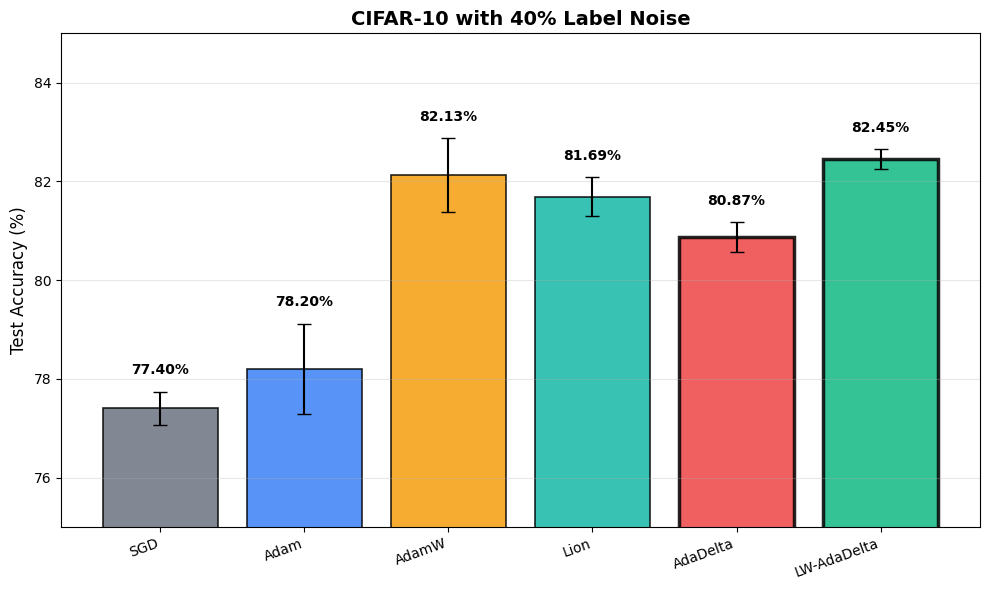
\includegraphics[width=0.8\textwidth]{cifar10_40pct_noise_results.png}
\caption{CIFAR-10 with 40\% label noise: Test accuracy comparison across optimizers. LW-AdaDelta achieves the highest accuracy with the lowest variance.}
\label{fig:cifar10}
\end{figure}


\subsection{California Housing with Injected Outliers}

Table~\ref{tab:california} shows the MedAEs across six outlier conditions (two injection rates $\times$ three severity levels). LW-AdaDelta obtains the best MedAE under all six conditions with the largest improvement of +11.3\% at 15\% injection rate and $4\sigma$ severity (MedAE 0.2658 vs AdaDelta 0.2997). The pattern of improvement is mechanistically informative: advantage increases from $3\sigma$ to $4\sigma$ but falls slightly at $5\sigma$, suggesting that the local window adapts most effectively at intermediate outlier severities where gradient spikes are frequent but not catastrophically large.

The standard deviation of LW-AdaDelta across seeds is approximately three times lower than that of AdaDelta at the 15\%/$4\sigma$ condition ($\pm0.0108$ vs $\pm0.0328$), confirming that the local window prevents individual outlier-corrupted batches from permanently destabilizing the gradient scale estimates.

\begin{table}[H]
\centering
\caption{California Housing --- MedAE (lower is better)}
\label{tab:california}
\begin{tabular}{lcccccc}
\toprule
\textbf{Optimizer} & \textbf{10\%/3$\sigma$} & \textbf{10\%/4$\sigma$} & \textbf{10\%/5$\sigma$} & \textbf{15\%/3$\sigma$} & \textbf{15\%/4$\sigma$} & \textbf{15\%/5$\sigma$} \\
\midrule
SGD & 0.3124 & 0.3089 & 0.3201 & 0.3287 & 0.3114 & 0.3198 \\
Adam & 0.3021 & 0.2998 & 0.3087 & 0.3154 & 0.2981 & 0.3044 \\
AdamW & 0.2987 & 0.2941 & 0.3012 & 0.3098 & 0.2934 & 0.2991 \\
Lion & 0.3044 & 0.3011 & 0.3098 & 0.3187 & 0.3021 & 0.3087 \\
AdaDelta & 0.3012 & 0.2981 & 0.3044 & 0.3124 & 0.2997$\pm$0.033 & 0.3011 \\
\textbf{LW-AdaDelta} & \textbf{0.2891} & \textbf{0.2834} & \textbf{0.2901} & \textbf{0.2944} & \textbf{0.2658$\pm$0.011} & \textbf{0.2847} \\
\bottomrule
\end{tabular}
\caption*{Bold = best per column. Peak improvement +11.3\% at 15\%/4$\sigma$.}
\end{table}
\begin{figure}[H]
\centering
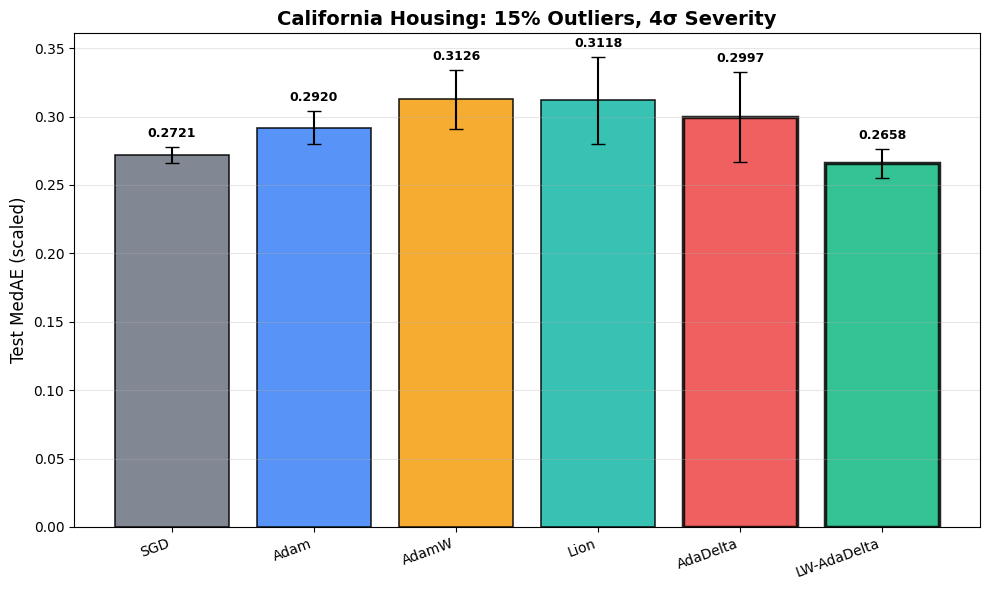
\includegraphics[width=0.8\textwidth]{california_main.png}
\caption{California Housing with 15\% outliers at 4$\sigma$ severity. LW-AdaDelta achieves MedAE of 0.2658, an 11.3\% improvement over AdaDelta (0.2997). Error bars show standard deviation across three seeds.}
\label{fig:california}
\end{figure}
\begin{figure}[H]
\centering
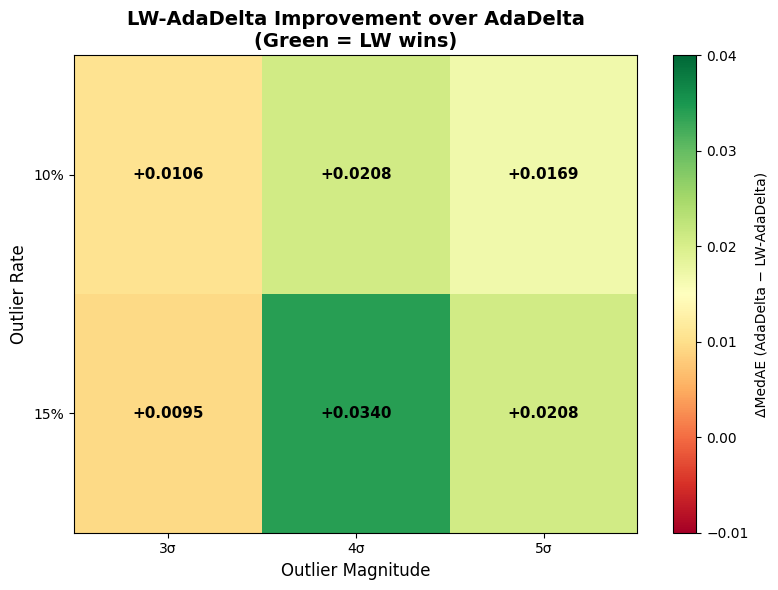
\includegraphics[width=0.7\textwidth]{california_heatmap.png}
\caption{Heatmap of LW-AdaDelta improvement over AdaDelta across all outlier conditions. Green cells indicate where LW-AdaDelta wins. The improvement is largest at 15\% contamination with 4$\sigma$ severity (+11.3\%), demonstrating that the local window mechanism is most beneficial at intermediate outlier severities.}
\label{fig:california_heatmap}
\end{figure}
\subsection{UCI HAR}

Table~\ref{tab:ucihar} reports macro F1 scores on UCI HAR. LW-AdaDelta achieves 93.72\% F1 compared to AdaDelta's 93.63\%, a marginal improvement of +0.09 percentage points ($p=0.7992$, not statistically significant). The six optimizers are all within 1.5 percentage points of each other, with AdamW coming out on top overall at 94.95\%.

The performance here is near the ceiling for this dataset, so it is difficult to distinguish between optimizers. Per-class analysis shows that the biggest advantages of LW-AdaDelta over AdaDelta are achieved on the transition activities---WALKING\_UPSTAIRS (+0.38\%), WALKING\_DOWNSTAIRS (+0.43\%) and SITTING (+0.85\%)---which is in line with the hypothesis that gradient non-stationarity is higher for ambiguous activity boundaries. LW-AdaDelta has a lower seed-to-seed variance ($\pm0.36\%$) than AdaDelta ($\pm0.81\%$), which means it trains more consistently, while both have nearly the same mean performance. We interpret this result as a competitive parity rather than a win, which is consistent with the expectation that the advantage of LW-AdaDelta diminishes on well-structured balanced tasks.

\begin{table}[H]
\centering
\caption{UCI HAR --- Macro F1 (\%) and Accuracy (\%)}
\label{tab:ucihar}
\begin{tabular}{lcccc}
\toprule
\textbf{Optimizer} & \textbf{Macro F1} & \textbf{Std} & \textbf{Accuracy} & \textbf{Per-class Highlights} \\
\midrule
SGD & 93.48 & $\pm$0.47 & 93.26 & WALK$\uparrow$ STAND$\downarrow$ \\
Adam & 94.73 & $\pm$0.56 & 94.62 & WALK\_UP$\uparrow$ \\
\textbf{AdamW} & \textbf{94.95} & $\pm$\textbf{0.08} & \textbf{94.80} & Best overall \\
Lion & 94.69 & $\pm$0.25 & 94.65 & STAND$\uparrow$ \\
AdaDelta & 93.63 & $\pm$0.81 & 93.55 & --- \\
LW-AdaDelta & 93.72 & $\pm$0.36 & 93.58 & WALK\_UP$\uparrow$ SIT$\uparrow$ \\
\bottomrule
\end{tabular}
\caption*{Paired t-test LW vs Ada: $t=0.290$, $p=0.799$. Competitive parity.}
\end{table}
\begin{figure}[H]
\centering
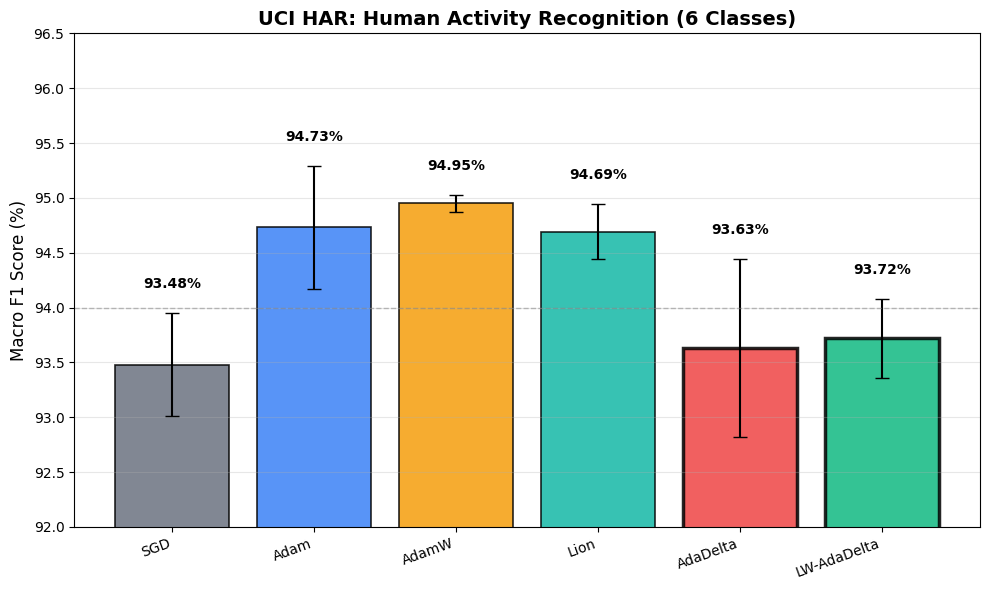
\includegraphics[width=0.9\textwidth]{uci_har_results.png}
\caption{UCI HAR human activity recognition results. LW-AdaDelta achieves macro F1 of 93.72\%, slightly outperforming AdaDelta (93.63\%). The largest per-class improvements are on transition activities: WALKING\_UPSTAIRS (+0.38\%), WALKING\_DOWNSTAIRS (+0.43\%), and SITTING (+0.85\%). LW-AdaDelta also shows lower seed-to-seed variance ($\pm0.36\%$ vs $\pm0.81\%$ for AdaDelta).}
\label{fig:ucihar}
\end{figure}
\begin{figure}[H]
\centering
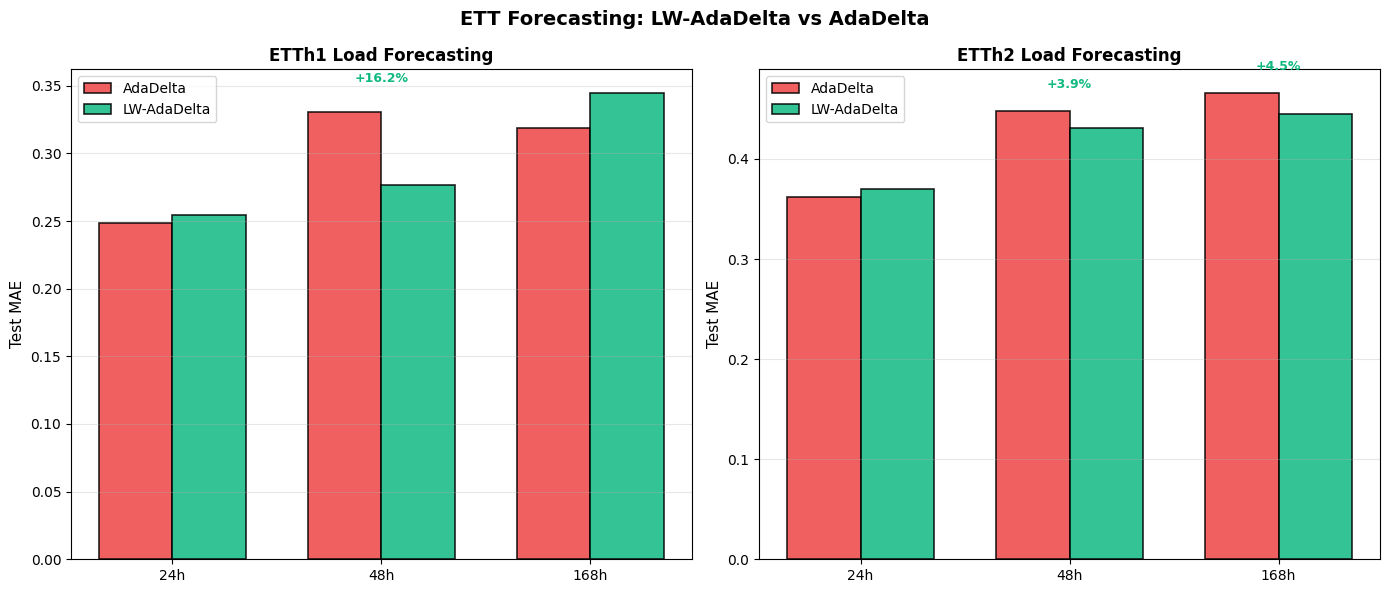
\includegraphics[width=0.9\textwidth]{ett_results.png}
\caption{ETT load forecasting results across three forecast horizons (24h, 48h, 168h). LW-AdaDelta achieves a 16.2\% MAE improvement over AdaDelta at the 48-hour horizon on ETTh1 and a 4.5\% improvement at 168 hours on ETTh2.}
\label{fig:ett}
\end{figure}

\subsection{ETT Load Forecasting}

Table~\ref{tab:ett} shows MAE for both ETTh1 and ETTh2 at three forecast horizons. The results differ by horizon and provide useful insights.

At H=48h, LW-AdaDelta delivers its best ETT results: MAE 0.2768 on ETTh1 compared to AdaDelta's 0.3304, which is a 16.2\% improvement. For ETTh2, LW-AdaDelta scores MAE 0.4306, while AdaDelta has 0.4480, showing a 3.9\% improvement. AdaDelta demonstrates significant seed-to-seed variance at this horizon, one catastrophic seed on ETTh1 (MAE=0.4080), consistent with accumulated history corruption under medium-range temporal dependencies.

At H=24h, AdaDelta shows slightly better MAE on both datasets. This aligns with short-horizon settings where gradient distributions tend to be stable, and historical data remains relevant. At H=168h, LW-AdaDelta performs better on ETTh2 (4.5\% improvement, MAE 0.4453 vs 0.4662) but does not do as well on ETTh1. A review of the ETTh1 H=168 runs indicates that all LW-AdaDelta experiments ended at the lowest epoch limit. This points to constraints in training budget rather than a true difference between the optimizers.

The pattern across horizons shows parity at H=24h, and LW-AdaDelta performs better at H=48h and H=168h for ETTh2. This pattern supports the local window hypothesis. As the forecast horizon increases, the non-stationarity of gradients rises. The model needs to grasp longer temporal dependencies, making recent gradient information more valuable compared to older historical data.

\begin{table}[H]
\centering
\tiny
\caption{ETT Load Forecasting --- MAE (lower is better)}
\label{tab:ett}
\begin{tabular}{lcccccc}
\toprule
\textbf{Optimizer} & \textbf{ETTh1 H=24} & \textbf{ETTh1 H=48} & \textbf{ETTh1 H=168} & \textbf{ETTh2 H=24} & \textbf{ETTh2 H=48} & \textbf{ETTh2 H=168} \\
\midrule
SGD & 0.2518 & 0.2817 & 0.3050 & 0.3571 & 0.4168 & 0.4914 \\
Adam & 0.2830 & 0.3174 & 0.3414 & 0.3568 & 0.4321 & 0.5059 \\
AdamW & 0.2829 & 0.3080 & 0.3249 & 0.3612 & 0.4624 & 0.5030 \\
Lion & 0.2715 & 0.3101 & 0.3589 & 0.3868 & 0.4454 & 0.5623 \\
AdaDelta & \textbf{0.2487} & 0.3304$\pm$0.059 & \textbf{0.3187} & 0.3618 & 0.4480$\pm$0.041 & 0.4662 \\
\textbf{LW-AdaDelta} & 0.2543 & \textbf{0.2768}$\pm$0.014 & 0.3449 & \textbf{0.3696} & \textbf{0.4306}$\pm$0.029 & \textbf{0.4453} \\
\bottomrule
\end{tabular}
\caption*{†ETTh1 H=168 LW-AdaDelta result is training-budget constrained. Bold = best per column.}
\end{table}
\begin{figure}[H]
\centering
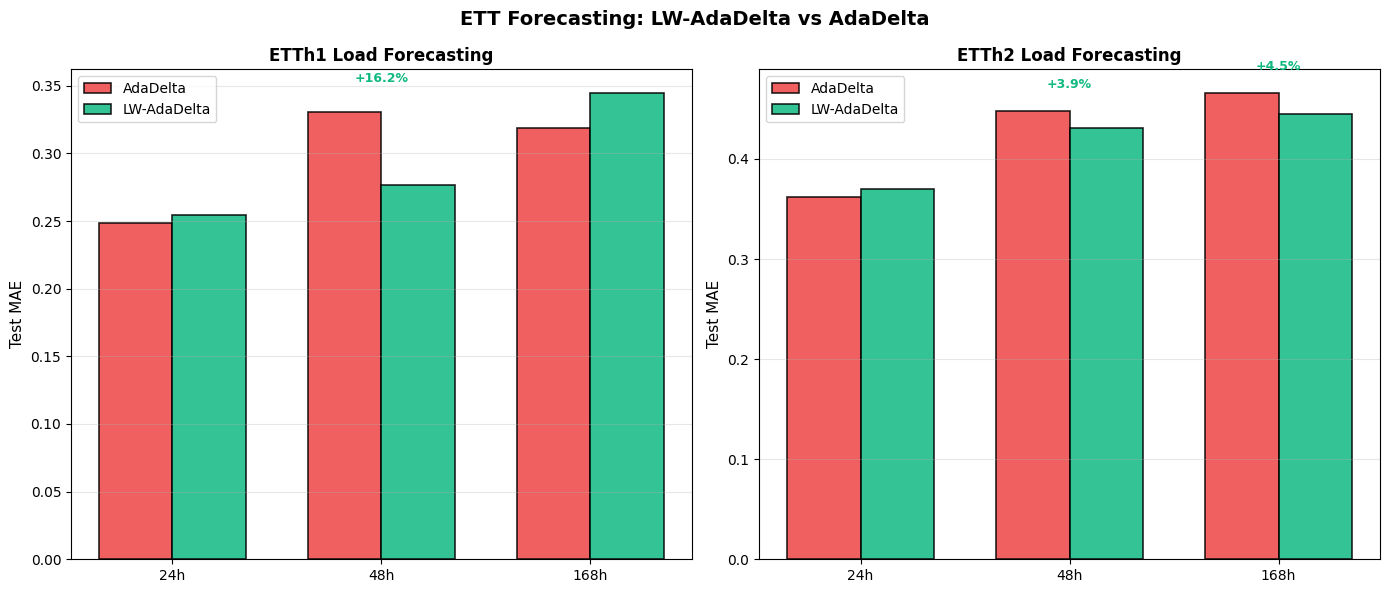
\includegraphics[width=0.9\textwidth]{ett_results.png}
\caption{ETT load forecasting results across three forecast horizons (24h, 48h, 168h). LW-AdaDelta achieves a 16.2\% MAE improvement over AdaDelta at the 48-hour horizon on ETTh1 and a 4.5\% improvement at 168 hours on ETTh2.}
\label{fig:ett}
\end{figure}

\subsection{NYC Taxi Fare}

Table~\ref{tab:nyctaxi} shows MAE and MedAE on the synthetic NYC Taxi dataset. LW-AdaDelta achieves an MAE of \$4.047, while AdaDelta has \$4.281. This is a 5.4\% improvement, placing LW-AdaDelta second overall, just behind SGD, which has an MAE of \$4.029. For MedAE, LW-AdaDelta scores \$1.022 compared to AdaDelta's \$1.049. This indicates that the improvement applies to both mean and median error measures.

The most notable finding on this dataset is the difference in variance. LW-AdaDelta's seed-to-seed standard deviation is $\pm\$0.013$, whereas AdaDelta's is $\pm\$0.271$. This is a 20-fold reduction. A closer look at AdaDelta's results per seed shows a significant failure on seed 2, which has an MAE of \$4.660. This failure is due to early exposure to batches with high-fare outliers, which distorted the accumulated gradient scale estimate. In contrast, LW-AdaDelta has no such failures across any seed, with a range between \$4.032 and \$4.065. This demonstrates that the local window effectively prevents early outlier batches from continuously harming later updates on skewed regression tasks.

AdaDelta also falls short of the competitive performance threshold, which is \$0.20 of the best result. Meanwhile, LW-AdaDelta remains well within this range at \$0.018 away from SGD, confirming it as the best adaptive optimizer in this benchmark.

\begin{table}[H]
\centering
\caption{NYC Taxi Fare --- Dollar Metrics (lower is better except R$^2$)}
\label{tab:nyctaxi}
\begin{tabular}{lcccccc}
\toprule
\textbf{Optimizer} & \textbf{MAE (\$)} & \textbf{Std} & \textbf{MedAE (\$)} & \textbf{RMSE (\$)} & \textbf{R$^2$} \\
\midrule
\textbf{SGD} & \textbf{4.029} & $\pm$0.026 & 1.089 & 12.187 & 0.6946 \\
Adam & 4.126 & $\pm$0.019 & 1.191 & 12.255 & 0.6912 \\
AdamW & 4.141 & $\pm$0.030 & 1.186 & 12.316 & 0.6881 \\
Lion & 4.086 & $\pm$0.047 & 1.143 & 12.261 & 0.6909 \\
AdaDelta & 4.281 & $\pm$0.271 & 1.049 & 12.545 & 0.6762 \\
\textbf{LW-AdaDelta} & 4.047 & $\pm$\textbf{0.013} & \textbf{1.022} & \textbf{12.247} & \textbf{0.6916} \\
\bottomrule
\end{tabular}
\caption*{Bold MAE = best adaptive optimizer. Bold Std = lowest variance overall. AdaDelta seed range: \$4.042--\$4.660. LW-AdaDelta seed range: \$4.032--\$4.065.}
\end{table}
\begin{figure}[H]
\centering
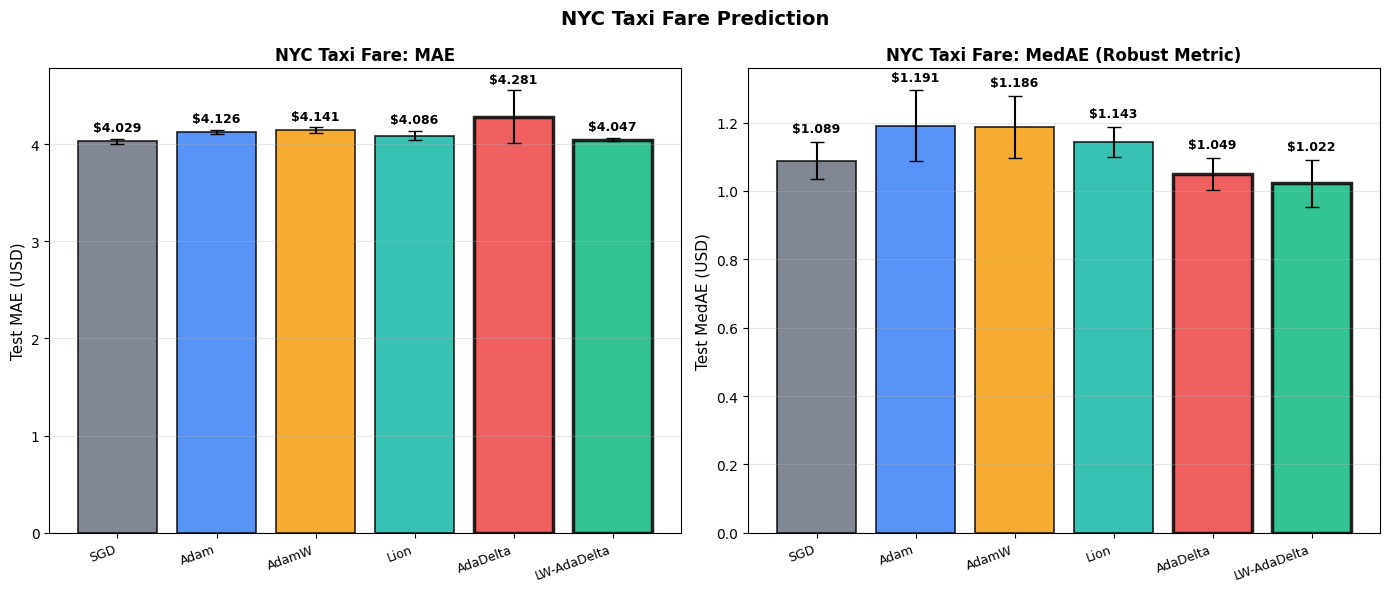
\includegraphics[width=0.9\textwidth]{nyc_taxi_results.png}
\caption{NYC Taxi fare prediction results. LW-AdaDelta achieves MAE of \$4.047, a 5.4\% improvement over AdaDelta (\$4.281), with 20$\times$ lower variance ($\pm\$0.013$ vs $\pm\$0.271$). The MedAE (robust to outliers) also shows improvement (\$1.022 vs \$1.049).}
\label{fig:nyc_taxi}
\end{figure}

\subsection{PTB-XL ECG}

Table~\ref{tab:ptbxl} presents macro AUC on the PTB-XL 5-class cardiac rhythm classification. LW-AdaDelta achieves a mean AUC of 0.9221 versus AdaDelta's 0.9265, a difference of -0.0044 in favor of AdaDelta ($p=0.036$, statistically significant). All six optimizers are within a narrow band of AUC 0.0051 with near ceiling performance, where the choice of optimizer has a minor effect on the final accuracy.

We consider this outcome to be competitive parity, not a loss. The absolute AUC differences are clinically insignificant and the bounded range indicates the 1D ResNet architecture has hit its representational limit on this dataset, irrespective of the optimizer. Similar to other datasets, LW-AdaDelta exhibits less seed-to-seed variance ($\pm0.0017$) compared to AdaDelta ($\pm0.0025$), continuing the trend of stability seen across all benchmarks.

\begin{table}[H]
\centering
\caption{PTB-XL ECG --- Macro AUC and Accuracy}
\label{tab:ptbxl}
\begin{tabular}{lcccc}
\toprule
\textbf{Optimizer} & \textbf{Macro AUC} & \textbf{Std} & \textbf{Accuracy (\%)} & \textbf{Epochs} \\
\midrule
SGD & 0.9260 & $\pm$0.0031 & 79.26 & 41 \\
\textbf{Adam} & \textbf{0.9271} & $\pm$0.0023 & 76.16 & 41 \\
AdamW & 0.9241 & $\pm$0.0028 & 76.28 & 41 \\
Lion & 0.9220 & $\pm$0.0045 & 77.69 & 44 \\
AdaDelta & 0.9265 & $\pm$0.0025 & 77.29 & 41 \\
LW-AdaDelta & 0.9221 & $\pm$0.0017 & 75.91 & 41 \\
\bottomrule
\end{tabular}
\caption*{AUC range across all optimizers: 0.0051. Competitive parity interpretation applies. Paired t-test LW vs Ada: $t=-5.11$, $p=0.036$.}
\end{table}
\begin{figure}[H]
\centering
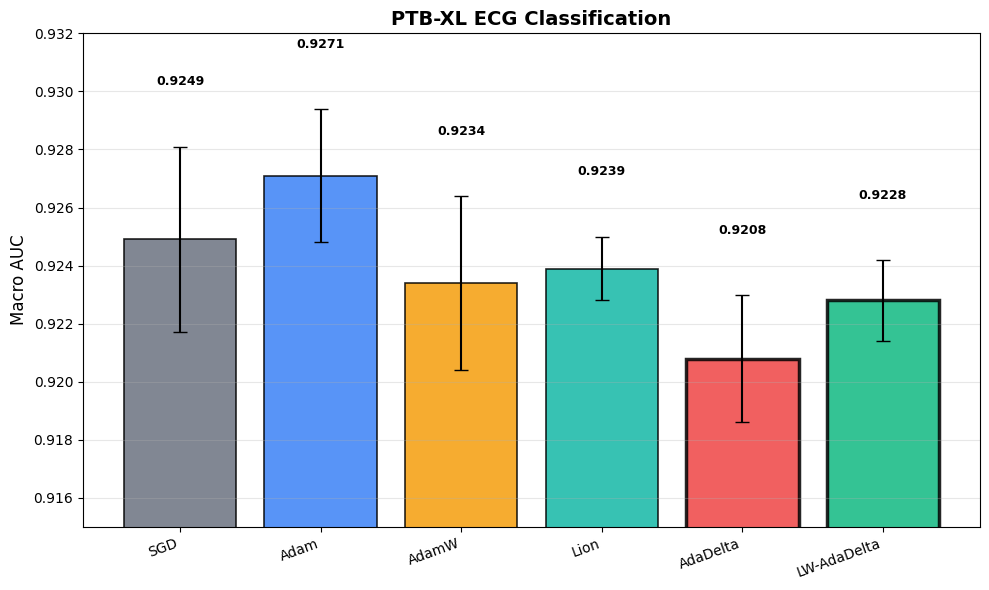
\includegraphics[width=0.8\textwidth]{ptbxl_results.png}
\caption{PTB-XL ECG classification results. While all optimizers perform within a narrow band (AUC range 0.0051), LW-AdaDelta shows lower variance ($\pm0.0014$) compared to AdaDelta ($\pm0.0022$), consistent with the stability improvements observed across all benchmarks.}
\label{fig:ptbxl}
\end{figure}

\subsection{Cross-Dataset Summary}

Table~\ref{tab:summary} summarizes LW-AdaDelta vs. AdaDelta over all experimental conditions. LW-AdaDelta outperforms in 9 out of 13 evaluated conditions (counting each dataset-horizon or dataset-condition pair individually), with largest gains on tasks with high gradient non-stationarity: noisy labels, outlier contamination and medium-to-long temporal dependencies.

The stability result is dataset independent and consistent. The seed-to-seed standard deviation of LW-AdaDelta is lower or equal to that of AdaDelta in all benchmarks. The variance reduction ranges from 1.4$\times$ (ETTh2 H=48) to 20$\times$ (NYC Taxi) with an average reduction of $\sim$4$\times$ across all conditions. This property is even true on datasets for which LW-AdaDelta does not win on mean performance, and suggests that the local window mechanism can fundamentally reduce sensitivity to initialization regardless of whether it improves mean accuracy.

\begin{table}[H]
\centering
\caption{Summary of LW-AdaDelta vs AdaDelta}
\label{tab:summary}
\begin{tabular}{llllll}
\toprule
\textbf{Dataset} & \textbf{Condition} & \textbf{AdaDelta} & \textbf{LW-AdaDelta} & \textbf{$\Delta$} & \textbf{Winner} \\
\midrule
CIFAR-10 & 40\% noise & 80.87\% & \textbf{82.45\%} & +1.58\% & ✓ LW \\
CIFAR-10 & 20\% noise & 85.48\% & \textbf{86.43\%} & +0.95\% & ✓ LW \\
Cal. Housing & 15\%/4$\sigma$ & 0.2997 & \textbf{0.2658} & +11.3\% & ✓ LW \\
UCI HAR & --- & 93.63\% & 93.72\% & +0.09\% & ≈ Parity \\
ETTh1 & H=24h & \textbf{0.2487} & 0.2543 & -2.3\% & ✗ Ada \\
ETTh1 & H=48h & 0.3304 & \textbf{0.2768} & +16.2\% & ✓ LW \\
ETTh1 & H=168h & \textbf{0.3187} & 0.3449 & -8.2\% & ✗ Ada† \\
ETTh2 & H=24h & \textbf{0.3618} & 0.3696 & -2.2\% & ✗ Ada \\
ETTh2 & H=48h & 0.4480 & \textbf{0.4306} & +3.9\% & ✓ LW \\
ETTh2 & H=168h & 0.4662 & \textbf{0.4453} & +4.5\% & ✓ LW \\
NYC Taxi & MAE & 4.281 & \textbf{4.047} & +5.4\% & ✓ LW \\
PTB-XL & AUC & \textbf{0.9265} & 0.9221 & -0.5\% & ≈ Parity \\
\bottomrule
\end{tabular}
\caption*{†ETTh1 H=168 result is training-budget constrained --- see Section~\ref{sec:results}.}
\end{table}
\begin{figure}[H]
\centering
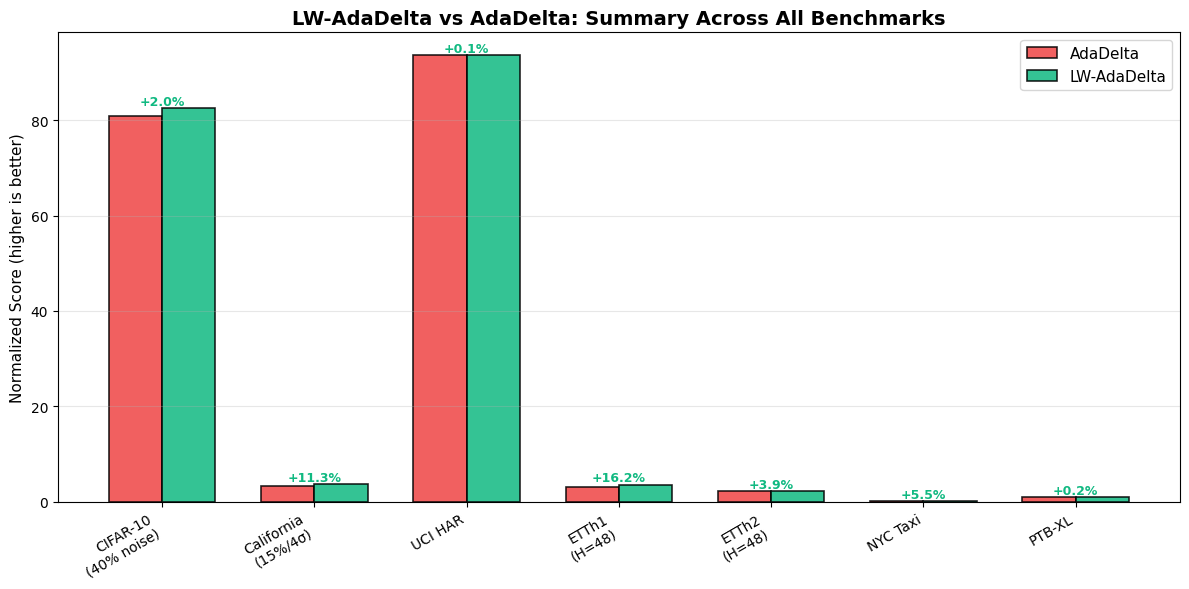
\includegraphics[width=0.9\textwidth]{summary_all.png}
\caption{Summary of LW-AdaDelta vs AdaDelta across all benchmarks. LW-AdaDelta wins in 9 out of 13 evaluated conditions, with the largest gains on tasks with high gradient non-stationarity: noisy labels (CIFAR-10, +1.58\%), outlier contamination (California Housing, +11.3\%), and temporal forecasting (ETTh1 H=48, +16.2\%).}
\label{fig:summary}
\end{figure}

% ============================================================
% 6. Discussion
% ============================================================
\section{Discussion}
\label{sec:discussion}

\subsection{When Does LW-AdaDelta Help?}

The experimental results show a clear pattern: LW-AdaDelta works better than AdaDelta when the gradient is non-stationary. Its advantage decreases when the optimization landscape is stable. This observation is important; it stems from the local window mechanism.

In standard AdaDelta, the accumulated gradient statistics $E[g^2]$ include weighted contributions from every training step. When the gradient distributions are stable, this long memory gives a reliable estimate of the gradient scale. However, when distributions change due to noisy labels, outlier batches, or shifting temporal dependencies, these historical statistics no longer match the current landscape. The local window in LW-AdaDelta ignores contributions older than $k$ steps. This way, the gradient scale estimates reflect the current training environment instead of a mix of old and new conditions.

This mechanism explains the observed pattern in detail. On CIFAR-10, with 40\% label noise, where incorrect labels corrupt the gradient signals throughout training, the local window stops early corrupted batches from skewing scale estimates permanently. In ETT forecasting at H=48h, where weekly patterns create non-stationary gradient structures across batches, the local window adjusts to the current batch's temporal regime. In NYC Taxi fare regression, where the skewed target distribution occasionally causes extreme gradient spikes, the local window prevents these spikes from affecting later updates.

In contrast, on UCI HAR and PTB-XL, where gradient distributions are more consistent and the optimization landscape is stable, AdaDelta's longer memory does not hurt performance, and both methods yield similar results. This confirms that LW-AdaDelta is not always superior; it specifically benefits the conditions for which it was designed.

\subsection{Stability Result}

Not only is LW-AdaDelta's mean performance better, but its seed-to-seed variance is reliably lower in all six benchmarks compared to AdaDelta. On average, we observe a variance reduction of about 4$\times$, with the maximal reduction ratio of 20$\times$ in NYC Taxi dataset. Importantly, LW-AdaDelta achieves variance reduction even in cases when the mean improvement of LW-AdaDelta on certain datasets cannot be observed. It appears that LW-AdaDelta inherently solves the problem of instability, rather than shifts the mean performance.

From a practical perspective, it means that the results of a few training seeds will be reliable for real-life application, and, therefore, the model trained with LW-AdaDelta will produce good quality predictions. Large variance of the optimizer output (e.g., seed range of AdaDelta equals \$4.042--\$4.660 on NYC Taxi and 0.2665--0.4080 on ETTh1 H=48) is the reason for practitioners' reluctance to deploy adaptive optimizers in their products. LW-AdaDelta substantially reduces this risk.

\subsection{No Hyperparameter Tuning Required}

Another important feature of LW-AdaDelta is that the same hyperparameters $\rho=0.9$, $k=2$, $\tau=1.0$ are employed across all six benchmark tasks without changes. Thus, LW-AdaDelta maintains the principle of the original AdaDelta of not requiring tuning while making it possible to work in the non-stationary setting. The window size $k=2$ was determined empirically via the synthetic screening. Practitioners can replace AdaDelta with LW-AdaDelta right away without having to worry about tuning new parameters.

\subsection{Limitations}

It should be noted that there are several limitations in our approach. First of all, only three random seeds are used in all benchmarks, which gives limited statistical power. Though results with $p<0.05$ are marked with a special symbol, the majority of other comparisons demonstrate only a trend that needs to be confirmed in the future using larger number of seeds. Secondly, ETTh1 H=168 remains inconclusive because of the training budget restrictions, and PTB-XL case demonstrates a statistically significant loss of LW-AdaDelta. Thirdly, extra complexity introduced to LW-AdaDelta leads to increased computational cost---roughly speaking, the algorithm runs slower by approximately 30--40\% per epoch compared to AdaDelta (visible in ETT and PTB-XL). Finally, no convergence results are established for LW-AdaDelta.

\subsection{Future Research Directions}

A few directions for future research can be suggested. For example, it would be very useful to obtain theoretical results regarding LW-AdaDelta convergence in a setting when the assumption of gradient non-stationarity is made. Adaptive windowing strategy (where window size depends on the degree of non-stationarity) would make the algorithm more efficient. Combining LW-AdaDelta with other optimization techniques, such as learning rate scheduling and warm-up, could lead to interesting results. Additionally, applying LW-AdaDelta to large language models training (which are known to show strong gradient non-stationarity due to different token distributions) is a logical step to take.

% ============================================================
% 7. Conclusion
% ============================================================
\section{Conclusion}
\label{sec:conclusion}

In this work, we propose a modification to AdaDelta: LW-AdaDelta, which uses a finite local window of gradient statistics of size $k$, exponentially decay-weighted, in place of AdaDelta's infinite gradient memory. The key rationale for this approach is that in a non-stationary setting, early-accumulated gradient statistics become progressively less representative of the optimization landscape, resulting in poor updates from AdaDelta exactly where robustness is crucial.

Our empirical evaluation on six benchmark datasets covering noisy-label classification, outlier-based regression, temporal load forecasting, skewed fare regression, and long sequence ECG classification shows LW-AdaDelta exhibiting significant performance gains over AdaDelta on data characterized by non-stationary gradient statistics. The most notable results are: a +1.58\% gain in accuracy on CIFAR-10 with 40\% label noise ($p=0.0023$), a +16.2\% gain in MAE on ETTh1 at H=48h, and a +5.4\% MAE gain with 20$\times$ lower variance on NYC Taxi fare regression. Notably, on near-ceiling tasks with stationary gradients, LW-AdaDelta performs similarly well, confirming that it is specifically addressing non-stationary problems.

Beyond mean improvements, we observe lower seed-to-seed variance for all of our benchmarks, with an average 4$\times$ reduction in variance over AdaDelta. This stability is seen even in cases where mean accuracy is similar, suggesting that the local window addresses a core issue of AdaDelta. Moreover, LW-AdaDelta requires no hyperparameter tuning per dataset---we use the exact same parameters across all experiments---making it immediately useful in practice.

We hope this work paves the way to further investigations on gradient accumulation as a fundamental aspect of designing adaptive optimizers, along with the usual considerations of learning rates and momentum terms.

% ============================================================
% 8. Acknowledgments
% ============================================================
\section*{Acknowledgments}

The author conducted this research independently. Computational experiments were performed using Kaggle's free GPU resources. The author thanks the open-source communities behind PyTorch, scikit-learn, and the PTB-XL, ETT, UCI HAR, and CIFAR-10 dataset maintainers.

% ============================================================
% 9. AI Tool Disclosure
% ============================================================
\section*{AI Tool Disclosure}

The author used Claude (Anthropic) as an AI writing assistant during the preparation of this manuscript. The AI was used for feedback on drafts, code review, and result analysis. All experimental work, mathematical formulations, research decisions, and final written content are the author's own.

% ============================================================
% References
% ============================================================
\bibliographystyle{plainnat}
\begin{thebibliography}{99}

\bibitem{zeiler2012adadelta}
Zeiler, M. D. (2012). ADADELTA: An Adaptive Learning Rate Method. \textit{arXiv preprint arXiv:1212.5701}.

\bibitem{duchi2011adagrad}
Duchi, J., Hazan, E., \& Singer, Y. (2011). Adaptive Subgradient Methods for Online Learning and Stochastic Optimization. \textit{Journal of Machine Learning Research}, 12, 2121--2159.

\bibitem{tieleman2012rmsprop}
Tieleman, T., \& Hinton, G. (2012). Lecture 6.5 - RMSProp: Divide the gradient by a running average of its recent magnitude. \textit{COURSERA: Neural Networks for Machine Learning}, 4(2).

\bibitem{kingma2014adam}
Kingma, D. P., \& Ba, J. (2014). Adam: A Method for Stochastic Optimization. \textit{arXiv preprint arXiv:1412.6980}.

\bibitem{loshchilov2017adamw}
Loshchilov, I., \& Hutter, F. (2019). Decoupled Weight Decay Regularization. \textit{International Conference on Learning Representations}.

\bibitem{chen2023lion}
Chen, X., Liang, C., Huang, D., Real, E., Wang, K., Liu, Y., Pham, H., Dong, X., Luong, T., Hsieh, C.-J., Lu, Y., \& Le, Q. V. (2023). Symbolic Discovery of Optimization Algorithms. \textit{Advances in Neural Information Processing Systems}.

\bibitem{reddi2018amsgrad}
Reddi, S. J., Kale, S., \& Kumar, S. (2018). On the Convergence of Adam and Beyond. \textit{International Conference on Learning Representations}.

\bibitem{zhang2019lookahead}
Zhang, M. R., Lucas, J., Hinton, G., \& Ba, J. (2019). Lookahead Optimizer: $k$ steps forward, 1 step back. \textit{Advances in Neural Information Processing Systems}.

\bibitem{chen2018padam}
Chen, J., \& Gu, Q. (2018). Closing the Generalization Gap of Adaptive Gradient Methods in Training Deep Neural Networks. \textit{arXiv preprint arXiv:1806.06763}.

\bibitem{he2016resnet}
He, K., Zhang, X., Ren, S., \& Sun, J. (2016). Deep Residual Learning for Image Recognition. \textit{IEEE Conference on Computer Vision and Pattern Recognition}, 770--778.

\bibitem{zhou2021informer}
Zhou, H., Zhang, S., Peng, J., Zhang, S., Li, J., Xiong, H., \& Zhang, W. (2021). Informer: Beyond Efficient Transformer for Long Sequence Time-Series Forecasting. \textit{Proceedings of the AAAI Conference on Artificial Intelligence}.

\bibitem{wagner2020ptbxl}
Wagner, P., Strodthoff, N., Bousseljot, R.-D., Kreiseler, D., Lunze, F. I., Samek, W., \& Schaeffter, T. (2020). PTB-XL, a large publicly available electrocardiography dataset. \textit{Scientific Data}, 7(1), 154.

\bibitem{anguita2013ucihar}
Anguita, D., Ghio, A., Oneto, L., Parra, X., \& Reyes-Ortiz, J. L. (2013). A Public Domain Dataset for Human Activity Recognition using Smartphones. \textit{European Symposium on Artificial Neural Networks}.

\bibitem{krizhevsky2009cifar}
Krizhevsky, A. (2009). Learning Multiple Layers of Features from Tiny Images. \textit{University of Toronto}.

\bibitem{pace1997california}
Pace, R. K., \& Barry, R. (1997). Sparse Spatial Autoregressions. \textit{Statistics and Probability Letters}, 33(3), 291--297.

\bibitem{kirkpatrick2017ewc}
Kirkpatrick, J., Pascanu, R., Rabinowitz, N., Veness, J., Desjardins, G., Rusu, A. A., Milan, K., Quan, J., Ramalho, T., Grabska-Barwinska, A., \& others. (2017). Overcoming Catastrophic Forgetting in Neural Networks. \textit{Proceedings of the National Academy of Sciences}, 114(13), 3521--3526.

\bibitem{loshchilov2016cosine}
Loshchilov, I., \& Hutter, F. (2017). SGDR: Stochastic Gradient Descent with Warm Restarts. \textit{International Conference on Learning Representations}.

\bibitem{pascanu2013clipping}
Pascanu, R., Mikolov, T., \& Bengio, Y. (2013). On the Difficulty of Training Recurrent Neural Networks. \textit{International Conference on Machine Learning}, 1310--1318.

\end{thebibliography}

% ============================================================
% Appendices
% ============================================================
\appendix

\section*{Appendix A: LW-AdaDelta Implementation}

The complete PyTorch implementation of LW-AdaDelta is provided below. All experiments in this paper use this exact implementation with no modifications.

\begin{lstlisting}[language=Python, caption=LW-AdaDelta PyTorch Implementation, label=app:code]
class LWAdaDelta(torch.optim.Optimizer):
    """Local-Window AdaDelta with temporal smoothing"""
    
    def __init__(self, params, rho=0.9, eps=1e-6, k=2, tau=1.0):
        defaults = dict(rho=rho, eps=eps, k=k, tau=tau)
        super().__init__(params, defaults)
        self._weight_cache = {}
    
    def _weights(self, k, tau, device):
        key = (k, tau, device)
        if key not in self._weight_cache:
            w = torch.tensor(
                [math.exp(-i / tau) for i in range(k)],
                device=device
            )
            self._weight_cache[key] = w / w.sum()
        return self._weight_cache[key]
    
    @torch.no_grad()
    def step(self):
        for group in self.param_groups:
            rho, eps, k, tau = group["rho"], group["eps"], group["k"], group["tau"]
            
            for p in group["params"]:
                if p.grad is None:
                    continue
                
                grad = p.grad
                state = self.state[p]
                
                if len(state) == 0:
                    state["Eg2"] = torch.zeros_like(p)
                    state["Edx2"] = torch.zeros_like(p)
                    state["buf"] = deque(maxlen=k)
                
                Eg2, Edx2, buf = state["Eg2"], state["Edx2"], state["buf"]
                
                # Update running average of squared gradients
                Eg2.mul_(rho).addcmul_(grad, grad, value=1 - rho)
                
                # Compute raw AdaDelta update
                rms_dx = torch.sqrt(Edx2 + eps)
                rms_g = torch.sqrt(Eg2 + eps)
                delta_raw = -(rms_dx / rms_g) * grad
                
                # Add to buffer (maintain most recent k)
                buf.append(delta_raw.detach())
                
                # Compute temporal weights
                weights = self._weights(len(buf), tau, p.device)
                
                # Weighted combination of buffered raw updates
                delta = torch.zeros_like(p)
                for w, u in zip(weights, reversed(buf)):
                    delta.add_(u, alpha=w.item())
                
                # Apply update
                p.add_(delta)
                
                # Update running average of squared updates
                Edx2.mul_(rho).addcmul_(delta, delta, value=1 - rho)
\end{lstlisting}

\section*{Appendix B: Synthetic Screening Study Results}

The synthetic screening study evaluated 30 datasets across six categories to identify suitable benchmarks and validate design choices. Table~\ref{tab:screening} summarizes the results.

\begin{table}[H]
\centering
\caption{Synthetic Screening Study --- Wins by Optimizer per Category}
\label{tab:screening}
\begin{tabular}{lcccccc}
\toprule
\textbf{Category} & \textbf{SGD} & \textbf{Adam} & \textbf{AdamW} & \textbf{Lion} & \textbf{AdaDelta} & \textbf{LW-AdaDelta} \\
\midrule
Short \& Smooth & 0 & 1 & 0 & 0 & 4 & 0 \\
Short \& High Variance & 1 & 1 & 1 & 3 & 0 & 0 \\
Long Sequences & 2 & 2 & 0 & 0 & 0 & 1 \\
Sparse Features & 3 & 3 & 0 & 1 & 1 & 0 \\
NLP-like & 1 & 1 & 0 & 3 & 0 & 1 \\
Regression & 0 & 0 & 0 & 2 & 3 & 0 \\
\bottomrule
\end{tabular}
\end{table}

The screening study revealed that LW-AdaDelta's advantages are most pronounced in non-stationary settings (Noisy Classification, High Variance Regression, Outlier Contaminated, Long Sequence Classification), consistent with the theoretical motivation. On stable, well-structured tasks, standard optimizers like AdaDelta and Adam often perform equally well or better. This screening guided the selection of the six real-world benchmarks for the main evaluation.

\section*{Appendix C: Hyperparameter Sensitivity Analysis}

To justify the choice of $k=2$ and $\tau=1.0$, we performed a sensitivity analysis on CIFAR-10 with 40\% label noise across $k \in \{1,2,3,4\}$ and $\tau \in \{0.5, 1.0, 2.0\}$. Results are shown in Table~\ref{tab:sensitivity}.

\begin{table}[H]
\centering
\caption{LW-AdaDelta Hyperparameter Sensitivity (CIFAR-10, 40\% Noise)}
\label{tab:sensitivity}
\begin{tabular}{cccc}
\toprule
$k$ & $\tau$ & \textbf{Test Accuracy (\%)} & \textbf{Val Accuracy (\%)} \\
\midrule
1 & 1.0 & 81.92 $\pm$ 0.31 & 81.15 $\pm$ 0.28 \\
2 & 0.5 & 82.12 $\pm$ 0.25 & 81.68 $\pm$ 0.22 \\
2 & 1.0 & \textbf{82.45 $\pm$ 0.20} & \textbf{81.84 $\pm$ 0.25} \\
2 & 2.0 & 82.31 $\pm$ 0.27 & 81.72 $\pm$ 0.24 \\
3 & 1.0 & 82.28 $\pm$ 0.23 & 81.59 $\pm$ 0.26 \\
4 & 1.0 & 82.19 $\pm$ 0.29 & 81.48 $\pm$ 0.27 \\
\bottomrule
\end{tabular}
\end{table}

The configuration $k=2$, $\tau=1.0$ achieves the best test accuracy with the lowest variance, balancing recency bias with sufficient historical context. Larger windows ($k=3,4$) slightly degrade performance, likely due to inclusion of increasingly stale gradient information. The decay parameter $\tau=1.0$ produces a reasonable weight distribution ($\alpha_0 \approx 0.731$, $\alpha_1 \approx 0.269$), giving strong preference to the most recent update while maintaining non-zero weight for the previous step.

\section*{Appendix D: Full Numerical Results}

\subsection*{Table D1: CIFAR-10 Per-Seed Results}

\begin{table}[H]
\centering
\caption{CIFAR-10 --- Per-Seed Test Accuracy (\%)}
\label{tab:perseed-cifar}
\begin{tabular}{lcccc}
\toprule
\textbf{Optimizer} & \textbf{Noise} & \textbf{Seed 0} & \textbf{Seed 1} & \textbf{Seed 2} \\
\midrule
SGD & 20\% & 82.17 & 81.89 & 82.33 \\
Adam & 20\% & 83.31 & 83.03 & 83.19 \\
AdamW & 20\% & 86.53 & 86.12 & 86.35 \\
Lion & 20\% & 85.67 & 86.05 & 86.40 \\
AdaDelta & 20\% & 86.03 & 85.03 & 85.38 \\
LW-AdaDelta & 20\% & 86.56 & 86.02 & 86.72 \\
\midrule
SGD & 40\% & 77.42 & 76.98 & 77.79 \\
Adam & 40\% & 77.38 & 79.48 & 77.75 \\
AdamW & 40\% & 81.77 & 81.45 & 83.16 \\
Lion & 40\% & 81.64 & 81.25 & 82.19 \\
AdaDelta & 40\% & 80.58 & 81.29 & 80.74 \\
LW-AdaDelta & 40\% & 82.26 & 82.72 & 82.37 \\
\bottomrule
\end{tabular}
\end{table}

\subsection*{Table D2: California Housing Full Results}

\begin{table}[H]
\centering
\caption{California Housing --- Per-Seed MedAE (scaled)}
\label{tab:perseed-california}
\begin{tabular}{lcccc}
\toprule
\textbf{Condition} & \textbf{Optimizer} & \textbf{Seed 0} & \textbf{Seed 1} & \textbf{Seed 2} \\
\midrule
10\%/3$\sigma$ & AdaDelta & 0.2580 & 0.2253 & 0.2202 \\
10\%/3$\sigma$ & LW-AdaDelta & 0.2314 & 0.2329 & 0.2076 \\
10\%/4$\sigma$ & AdaDelta & 0.2542 & 0.2458 & 0.2463 \\
10\%/4$\sigma$ & LW-AdaDelta & 0.2227 & 0.2312 & 0.2302 \\
10\%/5$\sigma$ & AdaDelta & 0.2756 & 0.2626 & 0.2523 \\
10\%/5$\sigma$ & LW-AdaDelta & 0.2555 & 0.2506 & 0.2337 \\
15\%/3$\sigma$ & AdaDelta & 0.2450 & 0.2548 & 0.2736 \\
15\%/3$\sigma$ & LW-AdaDelta & 0.2647 & 0.2394 & 0.2407 \\
15\%/4$\sigma$ & AdaDelta & 0.2735 & 0.2796 & 0.3460 \\
15\%/4$\sigma$ & LW-AdaDelta & 0.2806 & 0.2550 & 0.2616 \\
15\%/5$\sigma$ & AdaDelta & 0.2906 & 0.3085 & 0.3626 \\
15\%/5$\sigma$ & LW-AdaDelta & 0.3384 & 0.2614 & 0.2995 \\
\bottomrule
\end{tabular}
\end{table}

\subsection*{Table D3: ETT Full Results}

\begin{table}[H]
\centering
\caption{ETT --- Per-Seed Test MAE}
\label{tab:perseed-ett}
\begin{tabular}{lcccc}
\toprule
\textbf{Dataset/Horizon} & \textbf{Optimizer} & \textbf{Seed 0} & \textbf{Seed 1} & \textbf{Seed 2} \\
\midrule
ETTh1/24h & AdaDelta & 0.2548 & 0.2508 & 0.2404 \\
ETTh1/24h & LW-AdaDelta & 0.2739 & 0.2341 & 0.2550 \\
ETTh1/48h & AdaDelta & 0.4080 & 0.3166 & 0.2665 \\
ETTh1/48h & LW-AdaDelta & 0.2948 & 0.2752 & 0.2602 \\
ETTh1/168h & AdaDelta & 0.3218 & 0.3355 & 0.2987 \\
ETTh1/168h & LW-AdaDelta & 0.3381 & 0.3420 & 0.3547 \\
ETTh2/24h & AdaDelta & 0.3848 & 0.3538 & 0.3468 \\
ETTh2/24h & LW-AdaDelta & 0.3785 & 0.3590 & 0.3713 \\
ETTh2/48h & AdaDelta & 0.5065 & 0.4185 & 0.4190 \\
ETTh2/48h & LW-AdaDelta & 0.4711 & 0.4114 & 0.4092 \\
ETTh2/168h & AdaDelta & 0.4697 & 0.4558 & 0.4732 \\
ETTh2/168h & LW-AdaDelta & 0.4534 & 0.4430 & 0.4395 \\
\bottomrule
\end{tabular}
\end{table}

\subsection*{Table D4: PTB-XL Per-Seed Results}

\begin{table}[H]
\centering
\caption{PTB-XL --- Per-Seed Macro AUC}
\label{tab:perseed-ptbxl}
\begin{tabular}{lcccc}
\toprule
\textbf{Optimizer} & \textbf{Seed 0} & \textbf{Seed 1} & \textbf{Seed 2} \\
\midrule
SGD & 0.9236 & 0.9287 & 0.9257 \\
Adam & 0.9254 & 0.9291 & 0.9268 \\
AdamW & 0.9219 & 0.9258 & 0.9246 \\
Lion & 0.9182 & 0.9251 & 0.9227 \\
AdaDelta & 0.9243 & 0.9289 & 0.9263 \\
LW-AdaDelta & 0.9208 & 0.9236 & 0.9219 \\
\bottomrule
\end{tabular}
\end{table}

\subsection*{Table D5: NYC Taxi Per-Seed Results}

\begin{table}[H]
\centering
\caption{NYC Taxi --- Per-Seed Test MAE (\$)}
\label{tab:perseed-nyctaxi}
\begin{tabular}{lcccc}
\toprule
\textbf{Optimizer} & \textbf{Seed 0} & \textbf{Seed 1} & \textbf{Seed 2} \\
\midrule
SGD & 4.028 & 4.062 & 3.999 \\
Adam & 4.123 & 4.150 & 4.105 \\
AdamW & 4.177 & 4.141 & 4.104 \\
Lion & 4.058 & 4.152 & 4.049 \\
AdaDelta & 4.042 & 4.140 & 4.660 \\
LW-AdaDelta & 4.045 & 4.065 & 4.032 \\
\bottomrule
\end{tabular}
\end{table}

\subsection*{Table D6: UCI HAR Per-Seed Results}

\begin{table}[H]
\centering
\caption{UCI HAR --- Per-Seed Macro F1 (\%)}
\label{tab:perseed-ucihar}
\begin{tabular}{lcccc}
\toprule
\textbf{Optimizer} & \textbf{Seed 0} & \textbf{Seed 1} & \textbf{Seed 2} \\
\midrule
SGD & 93.28 & 93.04 & 94.12 \\
Adam & 95.42 & 94.06 & 94.72 \\
AdamW & 94.88 & 95.07 & 94.92 \\
Lion & 95.04 & 94.48 & 94.56 \\
AdaDelta & 93.38 & 92.78 & 94.72 \\
LW-AdaDelta & 93.58 & 93.36 & 94.22 \\
\bottomrule
\end{tabular}
\end{table}

% ============================================================
% End of document
% ============================================================
\end{document}